%%%% ijcai16.tex

\typeout{IJCAI-16 Instructions for Authors}

% These are the instructions for authors for IJCAI-16.
% They are the same as the ones for IJCAI-11 with superficical wording
%   changes only.

\documentclass{article}
% The file ijcai16.sty is the style file for IJCAI-16 (same as ijcai07.sty).
\usepackage{ijcai16}

\usepackage{tikz}
\usetikzlibrary{arrows,positioning,automata}
\usepackage[noend]{algpseudocode}
\usepackage{algorithm}
\usepackage{enumitem, kantlipsum}

% Use the postscript times font!
\usepackage{times}

\usepackage{mathtools}

% the following package is optional:
%\usepackage{latexsym} 

% Following comment is from ijcai97-submit.tex:
% The preparation of these files was supported by Schlumberger Palo Alto
% Research, AT\&T Bell Laboratories, and Morgan Kaufmann Publishers.
% Shirley Jowell, of Morgan Kaufmann Publishers, and Peter F.
% Patel-Schneider, of AT\&T Bell Laboratories collaborated on their
% preparation.

% These instructions can be modified and used in other conferences as long
% as credit to the authors and supporting agencies is retained, this notice
% is not changed, and further modification or reuse is not restricted.
% Neither Shirley Jowell nor Peter F. Patel-Schneider can be listed as
% contacts for providing assistance without their prior permission.

% To use for other conferences, change references to files and the
% conference appropriate and use other authors, contacts, publishers, and
% organizations.
% Also change the deadline and address for returning papers and the length and
% page charge instructions.
% Put where the files are available in the appropriate places.
% \thanks{These match the formatting instructions of IJCAI-07. The support of
% IJCAI, Inc. is acknowledged.}

\title{Relevance and Controllability Appraisals in Human-Robot Collaboration}
\author{Mahni Shayganfar, Charles Rich, Candace L. Sidner \\ 
Worcester Polytechnic Institute, Worcester Massachusetts  \\
mshayganfar $|$ rich $|$ sidner @wpi.edu}

\begin{document}

\maketitle

\begin{abstract}
We have investigated the mutual influence of affective and collaborative
processes in a cognitive theory to support interaction between humans and robots
or virtual agents. We have developed new algorithms for appraisal processes, as
part of a new overall computational model for implementing collaborative robots
and agents. We build primarily on the \textit{cognitive appraisal} theory of
emotions and the \textit{SharedPlans} theory of collaboration to investigate the
structure, fundamental processes and functions of emotions in a collaboration.
We have evaluated our implemented algorithms by conducting an online user study.
\end{abstract}

\section{Introduction}

Sousa in The Rationality of Emotion \cite{sousa:rationality-emotion}
makes the case for claiming that humans are capable of rationality largely
because they are creatures with emotions. The idea of having robots or other
intelligent agents living in a human environment has been a persistent dream
from science fiction books to artificial intelligence and robotics laboratories.
Collaborative robots are expected to become an integral part of humans'
environment to accomplish their industrial and household tasks. In these
environments humans will be involved in robots' operations and decision-making
processes. The involvement of humans influences the efficiency of robots'
interaction and performance, and makes them dependent on humans' cognitive
abilities and mental states.

This work is implemented as part of a larger effort to build robots capable of
generating and recognizing emotions in order to be better collaborators. In this
paper, we report on the specific problem of appraising events within a
collaborative interaction. Our contribution is to ground general appraisal
concepts in the specific context and structure of collaboration. This work is
part of the development of \textit{Affective Motivational Collaboration Theory}
which is built on the foundations of the \textit{SharedPlans} theory of
collaboration \cite{grosz:plans-discourse} and the \textit{cognitive appraisal}
theory of emotions \cite{gratch:domain-independent}.

After discussing related works, we briefly introduce the Affective Motivational
Collaboration Theory, focusing on the collaboration and appraisal mechanisms as
well as mental states. We then provide more details about the graph
representation of the robot's mental state. Next, we describe the algorithms we
developed to compute the value of four crucial appraisal variables. To compare
the results from our algorithms with humans' decisions we have conducted a user
study using crowd sourcing; the results are provided in Section
\ref{sec:user-study}.

\section{Related Work}

Our work builds on the general notions of appraisal theory
\cite{gratch:domain-independent,marsella:computational,scherer:sequential-appraisal-process,scherer:appraisal-processes},
but is focused on its application in human-robot collaboration. Computational
appraisal models have been applied to a variety of uses including psychology,
robotics, AI, and cognitive science. For instance, in
\cite{marsella:ema-process-model} EMA is used to generate specific predictions
about how human subjects will appraise and cope with emotional situations.
Furthermore, appraisal theory has also been used in robots' decision making
\cite{castro:autonomous-robot-fear}, or in their cognitive systems
\cite{hudlicka:emotinos-reasons,marinier:emotion-reinforcement}. Additionally,
in the virtual agents community, empathy and affective decision-making is a
research topic that has received much attention in the last two decades
\cite{scott:modeling-empathy-agent,paiva:agent-care,pontier:women-robot-men,velasquez:emotions-motivations-agents}.
However, EMA and several other examples in artificial intelligence and robotics
which apply appraisal theory do not focus on the dynamics of collaborative
contexts
\cite{adam:bdi-emotional-companion,kim:model-hri-appraisal,marsella:ema-process-model,rosenbloom:sigma-appraisal}.

The computational collaboration model in our work is strongly influenced by the
SharedPlans theory \cite{grosz:plans-discourse}. However, our algorithms are
also compatible with other collaboration theories, e.g., Joint Intentions theory
\cite{cohen:teamwork}, or STEAM \cite{tambe:flexible-teamwork}. These theories
have been extensively used to examine and describe teamwork and collaboration.
Yet, collaboration and emotion theories have never been combined, as they are in
our work. We believe a systematic integration of collaboration theories and
appraisal theory can help us describe the underlying collaboration processes
leading to the existing collaboration structures.

\section{{\fontsize{11.85}{12}\selectfont Affective Motivational Collaboration
Theory}}

Affective Motivational Collaboration Theory deals with the interpretation and
prediction of observable behaviors in a dyadic collaboration
\cite{shayganfar:appraisal-short}. The theory focuses on the processes regulated
by emotional states. The observable behaviors represent the outcome of reactive
and deliberative processes related to the interpretation of the self's
relationship to the environment. Affective Motivational Collaboration Theory
aims to explain both rapid emotional reactions to events as well as slower, more
deliberative responses. The reactive and deliberative processes are triggered by
two types of events: \textit{external} events, such as the other's
\textit{utterances} and \textit{primitive actions}, and \textit{internal}
events, comprising changes in the self's mental states, such as belief formation
and emotional changes. The theory explains how emotions regulate the underlying
processes when these events occur. It also elucidates the role of
\textit{motives} as goal-driven emotion-regulated constructs with which a robot
can form new intentions to cope with events.

\vspace*{-3mm}
\begin{figure}[tbh]
  \centering
  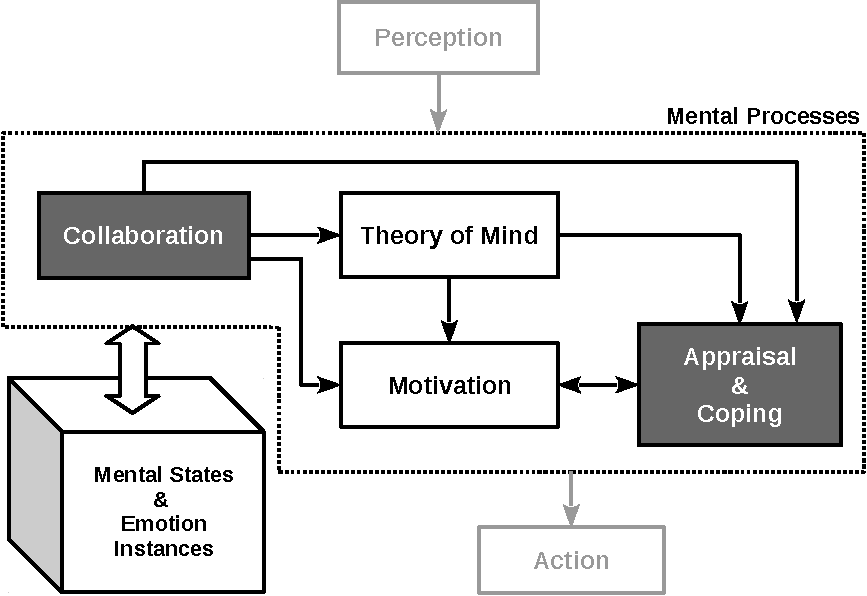
\includegraphics[width=0.45\textwidth]{figure/theory-general-croped.pdf}
  \vspace*{-3mm}
  \caption{{\fontsize{9}{9}\selectfont Computational framework based on
  Affective Motivational Collaboration Theory (arrows indicate primary
  influences between mechanisms).}}
  \vspace*{-3mm}
  \label{fig:cpm}
\end{figure}

Our focus is on the mechanisms depicted as mental processes in Figure
\ref{fig:cpm} along with the mental states. Each mechanism includes one or
more processes in our architecture. For instance, the \textit{Collaboration}
mechanism includes processes such as \textit{Focus Shifting} and
\textit{Constraint Management}, while as we discuss in Section
\ref{sec:appraisal-process} the \textit{Appraisal} mechanism includes processes
to compute the values for different appraisal variables. The \textit{mental
states} includes self's (robot's) beliefs, intentions, motives, goals and
emotion instances as well as the anticipated mental states of the other (human).
The \textit{Collaboration} mechanism maintains constraints on actions, including
task states and the ordering of tasks (see Figure \ref{fig:cs}). The
\textit{Collaboration} mechanism also provides processes to update and monitor
the shared plan. The \textit{Appraisal} mechanism is responsible for evaluating
changes in the self's mental states, the anticipated mental states of the other,
and the state of the collaboration environment. The \textit{Coping} mechanism
provides the self with different coping strategies associated with changes in
the self's mental states with respect to the state of the collaboration. The
\textit{Motivation} mechanism operates whenever the self a) requires a new
motive to overcome an internal impasse in an ongoing task, or b) wants to
provide an external motive to the other when the other faces a problem in a
task. The \textit{Theory of Mind} mechanism infers a model of the other's
anticipated mental state. The self progressively updates this model during the
collaboration.

\subsection{Mental States}
\label{sec:mental-states}

A brief description of mental states is provided as prerequisite knowledge for
understanding the appraisal processes. The mental states shown in Figure
\ref{fig:cpm} comprise the knowledge base required for all the mechanisms in the
overall model. Mental states are conscious states of mind providing the content
for cognitive processes. These mental states possess attributes, each of which
provides a unique interpretation of the related cognitive entities. The self
uses these attributes whenever there is an arbitration in the internal cognitive
processes. We only describe some of the attributes of beliefs and motives in
this paper, since they are used in our appraisal algorithms.

\textit{Beliefs} are a crucial part of the mental states. Beliefs have
attributes and they impact different processes of the framework such as the
evaluation of an external event by the Appraisal mechanism, and updates to the
collaboration plan. We use three belief attributes in in Appraisal mechanism.
Belief \textit{strength} is about how strongly the self holds salient beliefs
about an object, an entity, or an anticipated behavior. The \textit{saliency} of
a belief is a cognitive attribute that pertains to how easily the self becomes
aware of a belief. The \textit{persistence} of a belief refers to how resistant
the belief is to changes.

\textit{Motives} are mental constructs which can initiate, direct and maintain
goal-directed behaviors. They are created by the emotion-regulated Motivation
mechanism. Motives can cause the formation of a new intention for the robot
according to: a) its own emotional states, b) its own private goal, c) the
collaboration (shared) goal, and d) other's anticipated beliefs. Motives possess
a set of attributes. The Motivation mechanism compares motives based on the
quality of these attributes and chooses the one which is the most related to the
current state of the collaboration. We use two motive attributes in Appraisal
mechanisms. The \textit{importance} of a motive is determined by the
corresponding beliefs about the effects of achieving or not achieving the
associated goal. The \textit{urgency} of a motive defines how much time the self
has to acknowledge and address that motive before it is too late.

\textit{Intentions} are mental constructs directed at goals and future actions.
They play an essential role in taking actions according to the collaboration
plan as well as behavior selection in the Coping mechanism. Intentions are
also involved in selecting intention-related strategies, e.g., planning, seeking
instrumental support and procrastination. 

% Intentions possess a set of
% attributes, i.e., \textit{Temporal Status, Direct Experience, Certainty,
% Ambivalence, Affective-Deliberative Consistency} which moderate the consistency
% between intention and behavior \cite{cooke:intention-behavior-consistency}. The
% details about these attributes are beyond the scope of this paper.

\textit{Goals} help the robot to create and update its collaboration plan
according to the current private and shared goal content and structure. Goals
direct the formation of intentions to take appropriate corresponding actions
during collaboration. 

% Goals also drive the Motivation mechanism to generate
% required motive(s). The details about goal's attributes are beyond the scope of
% this paper.

\textit{Emotions} in mental states are emotion instances that are elicited by
the Appraisal mechanism, e.g., \textit{Joy, Anger, Hope, Worry}. These emotion
instances include the robot's own emotions as well as the anticipated emotions
of the other which are created with the help of the processes in the Theory of
Mind mechanism. 

% Each emotion has its own functionality in either the
% intrapersonal or interpersonal level. These emotions not only regulate the
% self's internal processes, but also assist the self to anticipate the other's
% mental states.

\begin{figure*}
  \centering
  \vspace*{-5mm}
  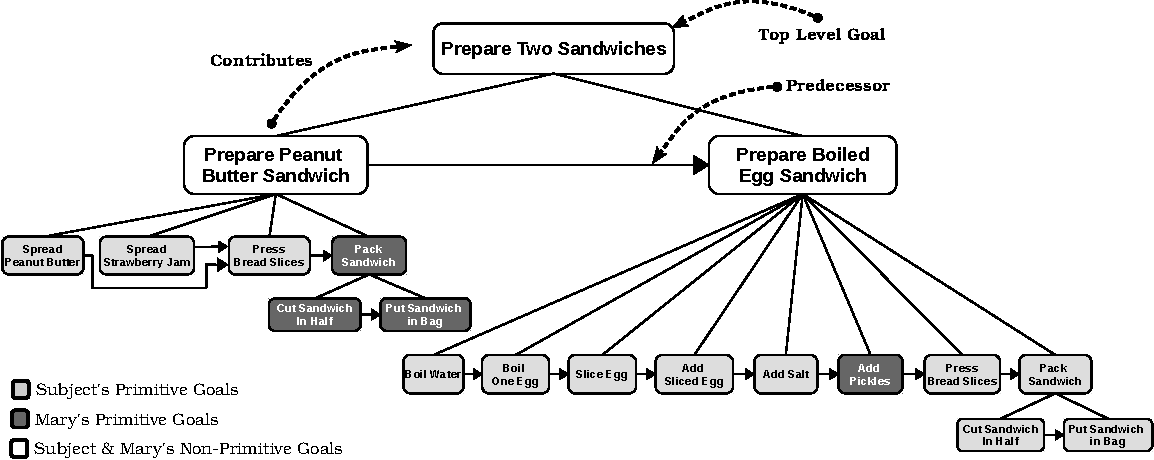
\includegraphics[width=16.5cm,height=6cm]{figure/taskModel-croped.pdf}
  \vspace*{-3mm}
  \caption{Collaboration structure (also used as task model for
  the evaluation).}
  \label{fig:taskModel}
  \vspace*{-4mm}
\end{figure*}

% \section{Example Scenario}
% 
% The example scenario is part of a much larger interaction we are implementing to
% test our theory. This example shows a very short part of an interaction between
% a robot and an astronaut during their collaboration. Their mission is to finish
% installing a few solar panels together. However, the astronaut encounters a
% measurement tool problem:
% 
% \begin{description}
%   \item \textit{\textbf{\fontsize{9pt}{12pt}\selectfont Astronaut [turn t-1]:}}
%   Oh no! Finishing the quality check of our installation with this measurement
%   problem is so frustrating. I think we should stop now!
% 
%   \item \textit{\textbf{\fontsize{9pt}{12pt}\selectfont{Robot [turn t]:}}}
%   I see. This is frustrating. But, I can help you with the measurement tool and
%   we can finish the task as originally planned.
% \end{description}
% 
% \vspace*{-1mm}
% In this scenario, the robot appraises the problem with the measurement tool as
% a \textit{relevant, undesirable, unexpected}, but \textit{controllable} event.
% Consequently, the coping mechanism first acknowledges the astronaut's negative
% valenced emotion (i.e., frustration), then provides a new plan to continue the
% collaboration.

\vspace*{-3mm}
\section{Collaboration}

The Collaboration mechanism constructs a hierarchy of goals associated with
tasks in the form of a hierarchical task network (see Figure
\ref{fig:taskModel}), and also manages and maintains the constraints and other
required details of the collaboration including the inputs and outputs of
individual tasks, the \textit{preconditions} (specifying whether it is
appropriate to perform a task), and the \textit{postconditions} (specifying
whether a just-completed task was successful). Collaboration also keeps track of
the focus of attention, which determines the salient objects, properties and
relations at each point, and shifts the focus of attention during the
interaction.

% \vspace*{-2mm}
% \begin{figure}[tbh]
%   \centering
%   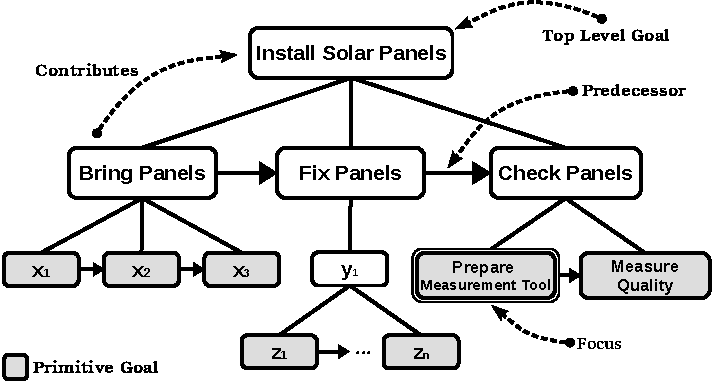
\includegraphics[width=0.474\textwidth]{figure/collaborationStructure-croped.pdf}
%   \vspace*{-4mm}
%   \caption{{\fontsize{9}{9}\selectfont Collaboration structure (shared plan).}}
%   \label{fig:cs}
%   \vspace*{-2mm}
% \end{figure}

Here, we briefly describe the methods which retrieve information about the
collaboration structure, and are used in our algorithms to compute the values of
appraisal variables. In these methods, $\varepsilon_t$ is the event
corresponding to time \textit{t}, and $g_t$ is a given goal at time \textit{t}.

\begin{itemize}[leftmargin=2pt]
  \setlength\itemsep{0.2mm}
  \item \textit{recognizeGoal($\varepsilon_t$)} returns the unique goal to which
  the given event (action, utterance, or emotional expression) directly
  contributes, or \textit{ambiguous} if this method does not recognize a goal in
  the plan.
  
  \item \textit{topLevelGoalStatus($g_t$)} returns the status of the top level
  goal whether it is \textsc{achieved, failed, blocked, inapplicable, pending,}
  or \textsc{in progress}.
  In our example, ``Prepare Two Sandwiches'' is the top level goal.
  
  \item \textit{currGoalStatus($g_t$)} returns the current goal status whether
  it is \textsc{achieved, failed, blocked, inapplicable, pending,} or \textsc{in
  progress}. In our example, ``Add Pickles'' is the current
  (focused) goal.
  
  \item \textit{precondStatus($g_t$)} returns the status of the precondition for
  the given goal whether it is \textsc{satisfied, unsatisfied} or
  \textsc{unknown}. For instance, the precondition for slicing the eggs is
  whether the eggs are boiled appropriately.
  
  \item \textit{isLive($g_t$)} returns \textit{true} if all the predecessors of
  the given goal are \textsc{achieved} and all the preconditions of the goal are
  \textsc{satisfied}; otherwise returns \textit{false}.
  
  \item \textit{isFocusShift($g_t$)} returns \textit{true} if the given
  goal is not the previous focus (top of the stack); otherwise returns
  \textit{false}.
  
  \item \textit{isNecessaryFocusShift($g_t$)} returns \textit{true} if the
  status of the previous focus was \textsc{achieved}; otherwise returns
  \textit{false} \cite{rich:focused-unfocused-users}.
  
  \item \textit{isPath($g_1$, $g_2$)} returns \textit{true} if there is a path
  between $g_1$ and $g_2$ in a plan tree structure; otherwise returns
  \textit{false}.
  
  \item \textit{doesContribute($g_t$)} returns whether the given goal
  contributes to another goal in the higher level of the plan hierarchy. For
  instance, an abstract (nonprimitive) goal of ``Prepare Peanut Butter
  Sandwich'' contributes to the higher level goal of ``Prepare Two Sandwiches''.
  
  \item \textit{extractContributingGoals($g_t$)} returns all the contributing
  goals of the given goal. For instance, ``Boil Water'', ``Boil Two Eggs'',
  ``Slice Eggs'' and other goals in this level are multiple goals contributing
  to the ``Prepare Boiled Egg Sandwich'' nonprimitive goal.
  
  \item \textit{extractPredecessors($g_t$)} returns the predecessors of the
  given goal. For instance, the ``Spread Peanut Butter'' and ``Spread
  Strawberry Jam'' goals are the predecessors of another goal called ``Press
  Bread Slices''.
  
  \item \textit{extractInputs($g_t$)} returns all the required inputs for
  the given goal. For example, the goal ``Boil Water'' requires inputs such as
  the \textit{Pot} and the \textit{Stove}.
  
  \item \textit{isAvailable($g_t$)} returns whether the given input is
  available. For instance, if the \textit{Pot} is required for the goal
  ``Boil Water'', is it available now?
  
  \item \textit{isAchieved($g_t$)} returns whether the given goal is achieved,
  i.e., whether all the postconditions of the given goal are \textsc{satisfied}.
  
  \item \textit{isFocused($g_t$)} returns whether the focus is on given
  goal now. In this example, the focus is on the goal ``Add Pickles''. The
  focused goal is the goal that the robot is currently pursuing.
  
  \item \textit{getResponsible($g_t$)} returns responsible agents of the given
  goal. In a dyadic collaboration, both of the agents can be partly responsible
  for a nonprimitive goal, while each is responsible for one or more primitive
  goals. For instance, both Mary and the subject are responsible for the
  nonprimitive goal of ``Prepare Peanut Butter Sandwich'', whereas it is only
  Mary who is responsible for the primitive goal of ``Spread Peanut Butter''.
\end{itemize}

\vspace*{-3mm}
\section{Appraisal Processes}
\label{sec:appraisal-process}

We discuss two appraisal variables in a collaboration context, i.e.,
\textit{Relevance} (since other appraisals are only derived for relevant
events), and \textit{Controllability} (since it is associated with the agent's
coping ability). There are other appraisal variables introduced in psychological
\cite{scherer:appraisal-processes} and computational literature
\cite{gratch:domain-independent}. We have implemented other appraisal variables
such as \textit{expectedness} \cite{shayganfar:appraisal-short} and
\textit{desirability} which do not appear in this paper due to the lack of
space. All of the algorithms in this section use mental states of the robot (see
Section \ref{sec:mental-states}) which are formed based on the collaboration
structure. All these algorithms use the corresponding recognized goal of the
most recent event at each turn.

\subsection{Relevance}

Relevance as an appraisal variable measures the significance of an event for the
robot. An event can be evaluated to be relevant if it has a non-zero utility
\cite{marsella:ema-process-model}. Relevance is an important appraisal variable
since the other appraisal variables are more meaningful only for relevant
events. However, the utility of an event during collaboration is influenced by
the other collaborator's actions and mental states while there is a commitment
between collaborators to achieve the shared goal based on the shared plan.
Whereas, other appraisal models only consider the utlity of an event only based
on the self's (robot's) goal and plan. 

Algorithm \ref{alg:relevance} determines the relevance of the given event with
respect to the current mental state. The relevance of the event depends on the
significance of the event with respect to the current collaboration status.
The significance of an event is determined based on the utility of the event as
it is also presented in
\cite{gratch:domain-independent,marsella:ema-process-model}. We believe
computing relevance of an event during collaboration involves some other factors
of which other appraisal models do not consider. For instance, the human's
perceived emotion (whether it is positive or negative), recurrence of a belief,
or occurrance of a belief about an unrelated goal by human also play an
important role by influencing the utility of an event during collaboration. As a
result, evaluating the relevance of the events can cause a collaborative robot
to respond effectively to the events which can positively impact the status of
the shared goal, without dedicating all resources to every single event.

\begin{algorithm}
	\caption{(Relevance)}
	\label{alg:relevance}
	\begin{algorithmic}[1]
		\Function{IsEventRelevant}{Event $\varepsilon_t$}
% 			\Statex
			\State $\mathit{g}_{t} \gets \textit{recognizeGoal}{(\varepsilon_t)}$
% 			\Statex
			\State $\mathcal{U} \gets \Call{getEventUtility}{\mathit{g}_{t}}$ 
			\State $\tau_{t} \gets \Call{getEmotionalThreshold}{\mathit{g}_{t}}$
% 			\Statex
			\If {$(  \tau_{t} \leq |\mathcal{U}| )$}
				\State \Return {{\fontsize{7}{8}\selectfont RELEVANT}}
			\Else
				\State \Return {{\fontsize{7}{8}\selectfont IRRELEVANT}}
			\EndIf
		\EndFunction
	\end{algorithmic}
\end{algorithm}

\vspace*{-3mm}
After perceiving an event, it is the belief about that event which represents
the event in the robot's mental state. Also, \textit{recognizeGoal} returns
the goal ($g_{t}$) to which the current event contributes, unless it is
\textit{ambiguous}; $g_{t}$ represents the shared goal at time (turn) $t$ within
the shared plan. We compute the utility ($-1 \leq \mathcal{U} \leq 1$) of the
event based on the values of the attributes associated with the existing
beliefs, as well as the attributes of the motive associated with the recognized
goal. We use three of the belief attributes discussed in Section
\ref{sec:mental-states} to compute the belief related part of the utility:

\vspace*{-1mm}
\begin{itemize}[leftmargin=2pt]
  \setlength\itemsep{0.2mm}
  \item \textit{Strength (T)}: The extent to which the preconditions ($\alpha$)
  and postconditions ($\beta$) of a goal and its predecessors ($\lambda$) and
  contributing goals ($\mu$) are \textsc{satisfied} or \textsc{unsatisfied}
  makes a belief about the goal stronger. Respectively, an \textsc{unknown}
  pre and postcondition status of a goal and its predecessors and contributing
  goals forms beliefs with lower strength. For instance, if one knows all
  predecessors of a pursuing goal (e.g., ``Press Bread Slices'' to make peanut
  butter sandwich) are \textsc{satisfied} (i.e., ``Spread Peanut Butter'' and
  ``Spread Strawberry Jam''), failure of the corresponding goal will elicit
  one's negative emotion (due to the strong beliefs related to the goal);
  whereas not knowing about the goal-related factors and status of a goal
  (e.g., whether Mary could find the knife to cut the sandwich in half) does not
  cause one to form strong beliefs about the goal.
  \item \textit{Saliency (S)}: Beliefs related to the goal at the top of the
  focus stack are more salient than beliefs related to any other goal in the
  plan, whether those goals are already \textsc{achieved} or \textsc{failed}, or
  they will be pursued in the future. For example, according to Figure
  \ref{fig:taskModel}, if one is making a peanut butter sandwich, some or all
  of the contributing goals to the ``Prepare Peanut Butter Sandwich'' (e.g.
  Spread Peanut Butter) will be in the focus stack (depending on the current
  goal), and consequently are more salient. Therefore, other goals in the other
  branches of the shared plan (e.g. Slice Egg) will not be salient.
  \item \textit{Persistence (P)}: The recurrence of a
  belief over the passage of time (turns) increases the persistence of the
  belief. Beliefs occurring only in one turn have the lowest value of
  persistence. For instance, if Mary keeps saying that she can not find the
  knife to cut the sandwich in half, although it is not part of the shared plan,
  one could pursue a new goal to acknowledge Mary's concern that can mitigate or
  prevent negative emotions.
\end{itemize}

\noindent We also use two motive attributes discussed in Section
\ref{sec:mental-states} to compute the motive related part of the utility
($\mathcal{U}$):

\begin{itemize}[leftmargin=2pt]
  \setlength\itemsep{1mm}
  \item \textit{Urgency ($\gamma$)}: There are two factors impacting the urgency
  of a motive: a) whether the goal directing the given motive is the predecessor of
  another goal for which the other collaborator is responsible, and b) whether
  achieving the goal directing the given motive can mitigate the other
  collaborator's negative valenced emotion. For instance, if one has a private
  goal to prepare (e.g. grabbing the eggs from the fridge) making the second
  sandwich while Mary is waiting to get the first sandwich and cut it in half,
  pressing bread slices and passing them to Mary will be more urgent than one's
  private goal.
  \item \textit{Importance ($\eta$)}: A motive is important if failure of the
  directing goal causes an impasse in the shared plan (i.e., no further goal is
  available to achieve), or achievement of the directing goal removes an
  existing impasse. For example, if one cannot find white bread to spread peanut
  butter (an impasse to make the peanut butter sandwich), and Mary offers to use
  wheat bread instead (external motive), the new motive becomes important for
  the one to remove the impasse on the shared plan.
\end{itemize}

\vspace*{-3mm}
\begin{equation}
    \Psi = \frac{\alpha_{_k} + \beta_{_k} + \lambda_{_k} +
    \mu_{_k}}{\alpha_{_{all}} + \beta_{_{all}} + \lambda_{_{all}} +
    \mu_{_{all}}} + \eta + \gamma
    \label{eqn:power}
\end{equation}

In equation \ref{eqn:power}, the subscript \textit{k} of the components of
the first term refers to the \textit{known} (\textsc{satisfied} or
\textsc{unsatisfied}) goal-related factors; whereas the subscript \textit{all}
includes both \textit{known} and \textit{unknown} goal-related factors.

\vspace*{-3mm}
\begin{equation}
    U(\varepsilon_t)= 
    \begin{dcases}
       P\cdot S^{\Psi} & \Psi \textgreater 0 \\
       0               & \Psi = 0
    \end{dcases}
    \label{eqn:utility}
\end{equation}

We compute the utility of an event based on these five attributes. The value of
each attribute is between -1 and 1, and we consider the same weight for each
attribute. These weights can be learned or modified when our framework is fully
implemented. The value of the overall utility is computed using a simple
weighted averaging function which results in an overall value between -1 and 1.

The significance of an event in a collaborative environment is based not
only on the utility of the event, but it is also influenced by the perceived
emotion of the human collaborator. The human's emotion influences the decision
about the utility of the event in the form of a threshold value $\tau_{t}$ (see
Algorithm \ref{alg:relevance}). For instance, a positively expressed emotion of
the human reduces the threshold value which consequently makes the robot find an
event relevant with even a slightly positive utility. This threshold value
($\tau_{t}$) is currently determined based on whether the valence of the
human's perceived emotion is positive (e.g., happiness) or negative (e.g.,
anger). Consequently, an event can be considered \textsc{irrelevant} even though
the utility has a relatively positive value, because relevance is influenced by
the human's perceived emotional state.

% \vspace*{-1mm}
% \subsection{Desirability}
% 
% Desirability characterizes the value of an event to the robot in terms of
% whether the event facilitates or thwarts the collaboration goal. Desirability
% captures the valence of an event with respect to the robot's preferences
% \cite{gratch:domain-independent}. In a collaborative robot, preferences are
% biased towards those events facilitating progress in the collaboration.
% Desirability plays an important role in the overall architecture; it makes the
% processes involved in the other mechanisms (e.g., Motivation and Theory of
% Mind), and consequently the robot's mental state, congruent with the
% collaboration status which is a collaborative robot's desire. Therefore, it
% causes the robot to dismiss events causing inconsistencies in the robot's
% collaborative behavior. Moreover, desirability is also crucial from the
% collaboration's point of view.
% 
% Algorithm \ref{alg:desirability} provides a process in which the desirability of
% an event is computed with regard to the status of the shared goal; i.e., it
% operates based on whether and how the event changes the status of the current
% shared goal. It distinguishes between the top level goal and the current goal
% because the top level goal's change of status attains a higher positive or
% negative value of desirability. For instance, failure of the top level goal
% (e.g., installing solar panel) is more undesirable than failure of a primitive
% goal (e.g., measuring the quality of the installed panel).
% 
% An \textsc{ambiguous} goal is a goal associated with the current event
% ($\varepsilon_t$) which is not recognized in the robot's plan; therefore it is
% \textsc{undesirable} for a collaborative robot. A top level goal' status must be
% \textsc{achieved} (i.e., \textsc{satisfied} postcondition) to consider the event
% \textsc{most-desirable}. When the goal's status is \textsc{failed} (i.e.,
% \textsc{unsatisfied} postcondition) or \textsc{blocked}, the associated event
% has the \textsc{most-undesirable} or \textsc{undesirable} values respectively.
% A goal is \textsc{blocked} if any of the required goals or goals recursively
% through the parent goal are not \textsc{achieved}. An \textsc{inapplicable} goal
% is also considered as \textsc{undesirable}. A goal is \textsc{inapplicable} if
% any of its predecessors are not \textsc{achieved}, and/or its preconditions are
% not \textsc{satisfied}. For \textsc{pending} and \textsc{inprogress} top level
% goals, the status of the current goal associated with the top level goal
% determines the status of the event $\varepsilon_t$. Only a non-primitive goal
% can have \textsc{inprogress} status, if it has been started but is not yet
% completed. A goal can be \textsc{pending} if it is live, or if it is a
% non-primitive goal that has not been started yet. \textsc{Achieved} current
% goals mark an event ($\varepsilon_t$) as \textsc{desirable}, while
% \textsc{failed} or \textsc{blocked} current goals render the event associated
% with them as \textsc{most-undesirable} and \textsc{undesirable} respectively.
% \textsc{Pending} or \textsc{inprogress} current goals mark their associated
% events as \textsc{neutral}.
% 
% \vspace*{-1mm}
% \begin{algorithm}
% 	\caption{(Desirability)}
% 	\label{alg:desirability}
% 	\begin{algorithmic}[1]
% 		\Function{IsEventDesirable}{Event $\varepsilon_t$}
% % 			\Statex
% 			\State $\mathit{g}_{t} \gets \textit{recognizeGoal}{(\varepsilon_t)}$
% % 			\Statex
% 			\If {$(\mathit{g}_{t} =$ {\fontsize{7}{8}\selectfont AMBIGUOUS}$)$} 
% 				\State \Return {\fontsize{7}{8}\selectfont UNDESIRABLE}
% 			\EndIf
% % 			\Statex
% 			\If {{\fontsize{8}{9}\selectfont(\textit{topLevelGoalStatus($g_{t}$)} =
% 			{\fontsize{7}{8}\selectfont ACHIEVED})}} 
% 			\State \Return {{\fontsize{7}{8}\selectfont MOST-DESIRABLE}} 
% 			\ElsIf {{\fontsize{8}{9}\selectfont(\textit{topLevelGoalStatus($g_{t}$)}} =
% 			{\fontsize{7}{8}\selectfont FAILED})} 
% 			\State \Return {{\fontsize{7}{8}\selectfont MOST-UNDESIRABLE}}
% 			\ElsIf {{\fontsize{8}{9}\selectfont(\textit{topLevelGoalStatus($g_{t}$)}} =
% 			{\fontsize{7}{8}\selectfont BLOCKED}) \OR\\
% 			\hspace{1mm}{\fontsize{8}{9}\selectfont
% 			\hspace*{4mm}(\textit{topLevelGoalStatus($g_{t}$)}} =
% 			{\fontsize{7}{8}\selectfont INAPPLICABLE)}} 
% 			\State \Return {{\fontsize{7}{8}\selectfont UNDESIRABLE}} 
% 			\ElsIf {{\fontsize{8}{9}\selectfont(\textit{topLevelGoalStatus($g_{t}$)}} =
% 			{\fontsize{7}{8}\selectfont PENDING}) \OR\\
% 			\hspace{1mm}{\fontsize{8}{9}\selectfont
% 			\hspace*{4mm}(\textit{topLevelGoalStatus($g_{t}$)}} =
% 			{\fontsize{7}{8}\selectfont INPROGRESS})}
% % 				\Statex
% 				\If {{\fontsize{8}{9}\selectfont (\textit{currGoalStatus($g_{t}$)}} =
% 				{\fontsize{7}{8}\selectfont ACHIEVED})}
% 				\State \Return {{\fontsize{7}{8}\selectfont DESIRABLE}}
% 				\ElsIf {(\textit{currGoalStatus($g_{t}$)} = {\fontsize{7}{8}\selectfont
% 				FAILED})} 
% 				\State \Return {{\fontsize{7}{8}\selectfont MOST-UNDESIRABLE}}
% 				\ElsIf {(\textit{currGoalStatus($g_{t}$)} = {\fontsize{7}{8}\selectfont
% 				BLOCKED}) \OR \\
% 				\hspace{1mm}{\fontsize{8}{9}\selectfont
% 				\hspace*{9mm}(\textit{topLevelGoalStatus($g_{t}$)}} =
% 				{\fontsize{7}{8}\selectfont INAPPLICABLE})} 
% 				\State \Return {{\fontsize{7}{8}\selectfont UNDESIRABLE}}
% 				\ElsIf {{\fontsize{8}{9}\selectfont(\textit{topLevelGoalStatus($g_{t}$)}} =
% 				{\fontsize{7}{8}\selectfont PENDING}) \OR \\ \hspace{1mm} 
% 				\hspace*{8mm}(\textit{currGoalStatus($g_{t}$)} =
% 				{\fontsize{7}{8}\selectfont INPROGRESS})} 
% 				\State \Return {{\fontsize{7}{8}\selectfont NEUTRAL}}
% 				\EndIf
% 			\EndIf
% 		\EndFunction
% 	\end{algorithmic}
% \end{algorithm}
% 
% \vspace*{-1mm}
% \subsection{Expectedness}
% 
% Expectedness is the extent to which the truth value of a state could have been
% predicted from causal interpretation of an event
% \cite{marsella:ema-process-model}. In the collaboration context the expectedness
% of an event evaluates the congruency of the event with respect to the existing
% knowledge about the shared goal. Thus, expectedness underlies a collaborative
% robot's attention. Congruent beliefs in a robot's mental state will lead to more
% consistent and effective outcomes of the processes in the overall architecture.
% The collaboration mechanism uses expectedness to maintain the robot's attention
% and subsequently its mental state with respect to the shared goal. Reciprocally,
% the appraisal mechanism uses the underlying information of the collaboration
% structure to evaluate the expectedness of an event. Therefore, a collaborative
% robot uses expectedness to maintain its own mental state towards the shared
% goal. The robot will also be able to respond to unexpected but relevant events.
% 
% \begin{algorithm}
% 	\caption{(Expectedness)}
% 	\label{alg:expectedness}
% 	\begin{algorithmic}[1]
% 		\Function{IsEventExpected}{Event $\varepsilon_t$}
% % 			\Statex
% 			\State $\mathit{g}_{t} \gets \textit{recognizeGoal}{(\varepsilon_t)}$
% 			\State $\mathit{g}_{top} \gets \textit{getTopLevelGoal}{(\mathit{g}_{t})}$
% % 			\Statex
% 			\If {$(\textit{isLive}{(\mathit{g}_{t})})$}
% 				\If {$(\neg \textit{isFocusShift}{(\mathit{g}_{t})}\hspace*{2mm}\OR$ \\
% 				\hspace*{13mm}$\textit{isNeccessaryFocusShift}{(\mathit{g}_{t})})$}
% 				\State \Return {\fontsize{7}{8}\selectfont MOST-EXPECTED}
% 				\Else
% 					\State \Return {\fontsize{7}{8}\selectfont EXPECTED}
% 				\EndIf
% 			\Else
% 				\If {$(\textit{isPath}{(\mathit{g}_{t}, \mathit{g}_{top})})$}
% 					\State \Return {\fontsize{7}{8}\selectfont UNEXPECTED}
% 				\Else
% 					\State \Return {\fontsize{7}{8}\selectfont MOST-UNEXPECTED}
% 				\EndIf
% 			\EndIf
% 		\EndFunction
% 	\end{algorithmic}
% \end{algorithm}
% 
% In Algorithm \ref{alg:expectedness} we provide the process of computing the
% expectedness based on the shared plan and status of the shared goal. The key
% point in this algorithm is the status of the current shared goal
% ($\mathit{g}_{t}$) that is associated with the event $\varepsilon_t$ and its
% relationship with the top level goal ($\mathit{g}_{_{top}}$).
% 
% The intuition captured here is that one expects the current goal to be finished
% before undertaking another activity, but the goals that are the next focus of
% attention are also to be expected \cite{rich:focused-unfocused-users}.
% Therefore, if the goal is live, the algorithm checks whether the goal has not
% changed, or the interpretation of the last event results in a necessary focus
% shift. Shifting the focus to a new goal is necessary when the former goal is
% achieved and a new goal is required. Consequently the new event is the
% \textsc{most-expected} one. However, even if the focus shift is not necessary,
% the new event can be considered as \textsc{expected}, since the corresponding
% goal is already live. For goals that have not yet been started (that is, are not
% live), the algorithm must determine how unexpected it would be to pursue one
% now; if the goal is at least in the plan, i.e., on the path to the top level
% goal, it is just \textsc{unexpected} while any others are
% \textsc{most-unexpected}.

\subsection{Controllability}
\label{sec:controllability}

Controllability is the extent to which an event can be influenced, and it is
associated with a robot's ability to cope with an appraised event
\cite{gratch:domain-independent}. Thus, a robot can determine whether the
outcome of an event can be altered by some actions under either of the
collaborators' control. In other words, controllability is a measure of a
robot's ability to maintain or change a particular state as a consequence of an
event.

\begin{algorithm}
	\caption{(Controllability)}
	\label{alg:controllability}
	\begin{algorithmic}[1]
		\Function{IsEventControllable}{Event $\varepsilon_t$}
% 			\Statex
			\State $\alpha \gets \Call{GetAgencyRatio}{\varepsilon_t}$ 
			\State $\beta \gets \Call{GetAutonomyRatio}{\varepsilon_t}$
% 			\Statex
			\State $\lambda \gets \Call{GetSucPredecessorsRatio}{\varepsilon_t}$
			\State $\mu \gets \Call{GetAvailableInput}{\varepsilon_t}$
% 			\Statex
			\State $\mathcal{U} \gets
			\frac{\omega_{0}\cdot \alpha + \omega_{1}\cdot \beta + \omega_{2}\cdot
			\lambda + \omega_{3}\cdot \mu}{\omega_{0} + \omega_{1} + \omega_{2} +
			\omega_{3}}$
% 			\Statex
			\State $\tau_{t} \gets \Call{getEmotionalThreshold}{ }$
% 			\Statex
			\If {$(\mathcal{U} \geq \tau_t)$}
				\State \Return {{\fontsize{7}{8}\selectfont CONTROLLABLE}}
			\Else
				\State \Return {{\fontsize{7}{8}\selectfont UNCONTROLLABLE}}
			\EndIf
		\EndFunction
	\end{algorithmic}
\end{algorithm}

\vspace*{-3mm}
Controllability is also important for the overall architecture. For instance,
the robot can choose to ask or negotiate about a collaborative task which is
not controllable, or the robot can interpret or predict the other's emotional
state (e.g., anger if the task is blocked, i.e., uncontrollable for the other),
or form a new motive to establish an alternative goal for the current
uncontrollable event. In general, other mechanisms in the architecture use the
appraisal process of controllability in their decision making processes;
meanwhile controllability uses the information from the collaboration structure,
e.g., successful predecessors of a goal.

An important determinant of one's emotional response is the sense of control
over the events occurring. This sense of subjective control is based on one's
reasoning about self's power. For instance, the robustness of one's plan for
executing actions can increase one's sense of power and subsequently the sense
of control. In the collaboration context, we have translated the sense of control
into a combination of four different factors including a) \textit{agency} and b)
\textit{autonomy} of the robot, as well as the ratios of c) \textit{successful
predecessors}, and d) the \textit{available inputs} of a given goal
(i.e., $\mathit{g}_{t}$) in the shared plan.

In Algorithm \ref{alg:controllability}, we compute the controllability of an
event based on these four factors (lines 2 to 5). We use weighted averaging over
these four factors to compute the utility of an event in terms of
controllability of the event. The value of all these weights are set to 1.0 for
the purpose of simplicity at this stage of the project. We will adjust these
weights after further investigating the influence of these factors, and
implementing other mechanisms in the overall architecture. After computing the
value of the utility, we compare this value to an emotional threshold similar to
what we discussed in Algorithm \ref{alg:relevance}. This comparison leads to our
decision about the controllability of an event (lines 8 to 11 in Algorithm
\ref{alg:controllability}).

\textit{\textbf{Agency}} is the capacity of an individual to act independently
in any given environment. In a collaborative environment collaborators are
sometimes required to act independently of each other. Hence, they need to have
some internal motives that are formed based on their own mental states rather
than motives that are reinforced by the other collaborator. These internal
motives will lead the collaborators to acquire new intentions towards new goals
whenever it is required. We extract the motive associated with the current goal
in the mental state. We consider a maximum agency value denoted as $\alpha$ in
Algorithm \ref{alg:controllability} (i.e., $\alpha=1.0$) if the robot's mental
state possesses an internal motive towards the recognized goal; otherwise we
consider the minimum agency value (i.e., $\alpha=0.0$) for no motives or
external motives only. Note that the process of forming new internal motives is
beyond scope of this paper.

\textit{\textbf{Autonomy}} is the ability to make decisions without the
influence of others. Autonomy implies acting on one's own and being responsible
for that. In a collaborative environment, tasks are delegated to the
collaborators based on their capabilities. Therefore, each collaborator is
responsible for the delegated task and the corresponding goal. In Algorithm
\ref{alg:controllability}, $\beta$ denotes the value of autonomy with regard to
the event ($\varepsilon_t$). This value is the ratio of the number of the goals
contributing to $\mathit{g}_{t}$ for which the robot is responsible over the
total number of contributing goals to $\mathit{g}_{t}$. If the goal associated
with the current event corresponds to a nonprimitive goal, the algorithm checks
the responsible agent for each primitive goal contributing to the nonprimitive
one and returns a value of which $(0 \leq \beta \leq 1)$. However, if the
associated goal of the current event corresponds to a primitive goal the value
of $\beta$ would be 0 or 1. In general, higher autonomy leads to a more positive
value of controllability.

The structure of a shared plan accommodates the order of the required
\textit{\textbf{predecessors}} of a goal. Predecessors of a goal, $g$, are other
goals that the collaborators should achieve before trying to achieve goal $g$.
We use the ratio of successfully achieved predecessors of the recognized goal
($\mathit{g}_{t}$) associated with the current event over the total number of
predecessors of the same goal. This ratio (denoted as $\lambda$ in Algorithm
\ref{alg:controllability}) is the third factor used to compute the
controllability of an event. If all of the predecessors of the given goal are
already achieved, then $\lambda=1$ which is the maximum value for $\lambda$. On
the contrary, failure of all of the predecessors will lead to $\lambda=0$.
Therefore, a higher $\lambda$ value positively impacts the value of
controllability for the current event.

Finally, \textit{\textbf{inputs}} of a task are the required elements that the
collaborators use to achieve the specified goal of the task. These inputs are
also part of the structure of a shared plan. We extract the required inputs of
the associated goal with the current event, and check whether all the required
inputs are available for the goal $\mathit{g}_{t}$. The outcome will be the
ratio of the available required inputs over the total required inputs of the
goal associated with the current event. This value (denoted as $\mu$ in
Algorithm \ref{alg:controllability}) will be bound to 0 and 1. Similar to the
other factors in the controllability process, the closer the value of $\mu$ gets
to 1, the more positive impact it has on the overall controllability value of
the event.

In summary, the output of these four appraisal processes serves as critical
input for the other mechanisms of the Affective Motivational Collaboration
Framework, shown in Figure \ref{fig:cpm}. By providing adequate interpretation
of events in the collaborative environment, the appraisal mechanism enables the
robot to carry out proper collaborative behaviors.

\vspace{-2mm}
\section{Evaluation}
\label{sec:user-study}

We developed our user study to test our hypothesis that humans will provide
similar answers as our algorithms to questions related to different factors used
to compute four appraisal variables. We conducted a between subject user study
using an online crowdsourcing website --
CrowdFlower\footnote{http://www.crowdflower.com}. We had one group of
subjects for each questionnaire corresponding to an appraisal variable.
There were 12 questions (including 2 test questions) in the controllability and
expectedness questionnaires, 14 questions (including 2 test questions) in
the desirability questionnaire, and 22 questions (including 3 test questions) in
the relevance questionnaire. Each group originally had 40 subjects. To increase
the quality of our subjects' answers, we limited the visibility of our
questionnaires to a few English speaking countries, i.e., United States,
Britain, and Australia. We also limited our subject pools to those that have
acquired the highest confidence level on the crowdsourcing website. Our
questionnaires included 2 or 3 test questions (depending on the length) to check
the sanity of the answers. We eliminated subjects providing wrong answers to our
sanity questions. We also eliminated subjects with an answering time less than 2
minutes. The number of accepted subjects in each group is provided in Table
\ref{tbl:statistics}.

\begin{table}[htbp]
\centering
\vspace*{-5mm}
\caption{Evaluation Results}
\begin{tabular}{|c|c|c|c|c|} \hline
{\fontsize{7.5}{8}\selectfont appraisal variables} &
{\fontsize{7.5}{8}\selectfont \# of subjects} & {\fontsize{8}{8}\selectfont
mean} & {\fontsize{7.5}{8}\selectfont stdev} &
{\fontsize{7.5}{8}\selectfont\textit{p}-value}\\ \hline 
{\fontsize{7.5}{8}\selectfont Relevance} & {\fontsize{7.5}{8}\selectfont 29} &
{\fontsize{7.5}{8}\selectfont 0.713} & {\fontsize{7.5}{8}\selectfont 0.107} &
{\fontsize{7.5}{8}\selectfont \textless0.001}\\ \hline {\fontsize{7.5}{8}\selectfont
Desirability} & {\fontsize{7.5}{8}\selectfont 35} &
{\fontsize{7.5}{8}\selectfont 0.778} & {\fontsize{7.5}{8}\selectfont 0.150} &
{\fontsize{7.5}{8}\selectfont \textless0.001}\\
\hline 
{\fontsize{7.5}{8}\selectfont Expectedness} & {\fontsize{7.5}{8}\selectfont 33}
& {\fontsize{7.5}{8}\selectfont 0.785} & {\fontsize{7.5}{8}\selectfont 0.120} &
{\fontsize{7.5}{8}\selectfont \textless0.001}\\
\hline 
{\fontsize{7.5}{8}\selectfont Controllability} & {\fontsize{7.5}{8}\selectfont
33} & {\fontsize{7.5}{8}\selectfont 0.743} & {\fontsize{7.5}{8}\selectfont
0.158} & {\fontsize{7.5}{8}\selectfont \textless0.001}\\
\hline
\end{tabular}
\vspace*{-2mm}
\label{tbl:statistics}
\end{table}

To minimize the background knowledge necessary for our test subjects, we used a
simple domestic example of preparing a peanut butter and jelly sandwich, and a
hard boiled egg sandwich for a hiking trip. We provided clear textual and
graphical instructions for all four questionnaires. The instructions presented
a sequence of hypothetical collaborative tasks to be carried out by the test
subject and an imaginary friend, Mary, in order to accomplish their goal of
preparing two sandwiches. Figure \ref{fig:taskModel} shows the corresponding
task model for these instructions. Test questions introduced specific situations
related to the shared plan; these situations included, among others, blocked
tasks, and failure or achievement of a shared goal provided in the instruction.
Each question provided three possible answers (which were counterbalanced in
the questionnaire). One option provided a distinct alternative; another option
was used to provide a dichotomy with the first alternative, and a third option
was used to check whether the subjects perceived the other two options as equal.
We also provided a brief description as well as a simple example for each
appraisal variable, e.g., \textit{relevance}, at the end of the corresponding
instructions. Using this approach, we prepared four different online
questionnaires for the appraisal variables: \textit{relevance, desirability,
expectedness} and \textit{controllability}. Note that the collaboration
structure and the instructions were the same for all four questionnaires.

Each question was designed based on different factors that we use in our
algorithms (see Section \ref{sec:appraisal-process}). Here, we present one
example question from the relevance questionnaire, and describe how this
question relates to a specific factor within the corresponding algorithm. The
input for our algorithms was the task model depicted in Figure
\ref{fig:taskModel}.

\begin{figure}[tbh]
  \vspace{-1mm}
  \centering
  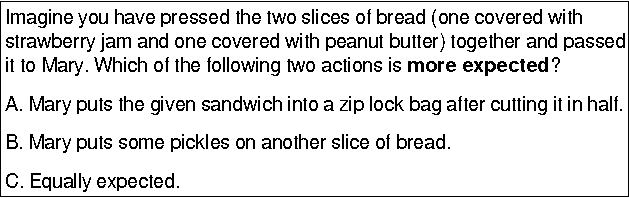
\includegraphics[width=0.48\textwidth]{figure/question-sample-croped.pdf}
  \vspace*{-7mm}
  \caption{{\fontsize{9}{9}\selectfont Example Expectedness Question.}}
  \label{fig:qs1}
  \vspace{-2mm}
\end{figure}

Figure \ref{fig:qs1} shows the example question from the relevance
questionnaire. In this example, with respect to Algorithm \ref{alg:relevance}
(line 6), option A is relevant because {\color{red}the task related to this
option provides the next available task in the focus stack (see the task model in
Figure \ref{fig:taskModel}). Although the task in option B is part of the
existing task model, it is considered as irrelevant by our algorithm, since it
is not live in the plan.} We provided option C to determine whether the human
subjects will similarly differentiate between these two options. This question
was presented to the human subjects to determine whether their decision for the
relevance of this event is similar to the output of the relevance algorithm. For
this question, the human decision was {\color{red}97\%} similar to the
algorithm's output. Average results for the relevance questionnaire are
presented in Table \ref{tbl:statistics}.

% \begin{figure}[tbh]
%   \vspace{-1mm}
%   \centering
%   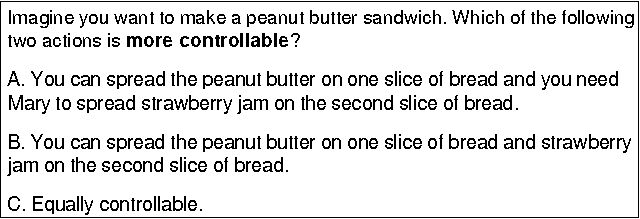
\includegraphics[width=0.48\textwidth]{figure/question-sample2-croped.pdf}
%   \vspace*{-7mm}
%   \caption{{\fontsize{9}{9}\selectfont Example Controllability Question.}}
%   \label{fig:qs2}
%   \vspace{-2mm}
% \end{figure}
% 
% Figure \ref{fig:qs2} shows an example question from the controllability
% questionnaire. The algorithm's output is option B, and is determined by
% Algorithm \ref{alg:controllability} (line 3), similarly to the expectedness
% example above. In this example, option B is more controllable than option A,
% because the self over total ratio of the responsibility of the predecessors of
% the given task (see \textit{Autonomy} in Section \ref{sec:controllability}) is
% higher than the ratio in option A; i.e., self is responsible to spread peanut
% butter on one slice of bread and strawberry jam on another slice of bread. In
% this question, the humans decision was 90\% in agreement with the algorithm's
% output.

% \begin{figure}[tbh]
%   \vspace{-1mm}
%   \centering
%   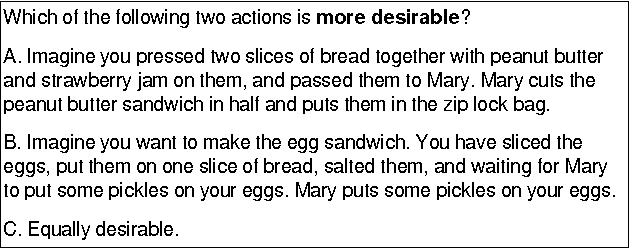
\includegraphics[width=0.48\textwidth]{figure/question-sample3-croped.pdf}
%   \vspace*{-7mm}
%   \caption{{\fontsize{9}{9}\selectfont Example Desirability Question.}}
%   \label{fig:qs3}
%   \vspace{-2mm}
% \end{figure}
% 
% Figure \ref{fig:qs3} shows an example question from the desirability
% questionnaire. The output based on the Algorithm \ref{alg:desirability}
% (line 14) is option C, since in both option A and option B, the focus goal
% has been achieved successfully. Therefore, in this example, both options A and B
% are desirable. The humans decision was 77\% in agreement with the algorithm's
% output in this question.

\vspace{-3mm}
\section{Discussion}
\vspace{-1mm}
We conducted the user study to compare the results with the implemented
algorithms discussed in Section \ref{sec:appraisal-process}. As we mentioned,
each question had 3 answers. Therefore, a totally random distribution would
result in 33\% agreement with our algorithms results. However, the average
ratio indicating similarity between human subjects decisions and the output of
our algorithms is significantly higher than 33\%. The total number of subjects'
answers similar to a) the \textit{relevance} algorithm (n=29) averaged 71.3\%
(s=10.7\%), b) the \textit{desirability} algorithm (n=35) averaged 77.8\%
(s=15.0\%), c) the \textit{expectedness} algorithm (n=33) averaged 78.5\%
(s=12.0\%), and d) the \textit{controllability} algorithm (n=33) averaged 74.3\%
(s=15.8\%). It is worth noting that the human subjects agreed 100\% on some
questions, while one some other questions there was a much lower level of
agreement.

The results indicate that our algorithms provide appraisal variable outputs
sufficiently similar to the decisions of human's appraisal. Our hypothesis in
our evaluation was that our algorithms would correctly predict the judgements of
humans on doing these tasks. Our results indicate that people largely performed
as our hypothesis predicted. The \textit{p}-values obtained based on a
one-tailed z-test (see Table \ref{tbl:statistics}) show the probability of human
subjects' data being generated from a random set. The very small
\textit{p}-values indicate that the data set is not random; in fact, the high
percentage of similarity shows that the four appraisal algorithms predicted the
human judgments.

\vspace{-2mm}
\section{Conclusion}
\vspace{-1mm}
While these results support our hypothesis, they are not a perfect prediction.
We believe the difference between these two results could be due to several
reasons, including: a) the fact that we conducted our study online and had
little control on our subjects, b) our algorithms may require further
granularity, or c) the difference between decision making processes of
individuals, which can be affected by other factors such as personality, gender,
and culture. While it may be possible to achieve a higher level of agreement
between humans and the algorithms results, these results indicate that the
current algorithms are adequate to be used in a collaboration context. In our
future work, we will implement the remaining mechanisms in Affective
Motivational Collaboration framework and carry out an end-to-end user study to
verify the behavior of a collaborative robot using our architecture.

\vspace*{-3mm}
\section*{Acknowledgments}
\vspace{-2mm}
{\fontsize{8.2}{9}\selectfont This work is supported by the National Science
Foundation under award IIS-1012083. Any opinions, findings, and conclusions
expressed in this material are those of the authors and do not necessarily
reflect the views of the National Science Foundation.}

%% The file named.bst is a bibliography style file for BibTeX 0.99c
\bibliographystyle{named}
\bibliography{mshayganfar}

\end{document}

